\documentclass[12pt]{report}
\usepackage[french]{babel}
\usepackage[utf8]{inputenc}
\usepackage[T1]{fontenc}
\usepackage[top=2cm, bottom=2cm, left=2cm, right=2cm]{geometry}
\usepackage{graphicx}
\usepackage{xcolor}
\usepackage{float}
\usepackage[french, onelanguage, boxruled, longend]{algorithm2e}
\usepackage{setspace}
\usepackage{multirow}
\usepackage{minted}
\usepackage[norelsize, linesnumbered, ruled, lined, boxed, commentsnumbered]{algorithm2e}

\newcommand{\HRule}{\rule{\linewidth}{0.5mm}}

\begin{document}
    \begin{titlepage}
        \begin{center}
            \textbf{République Algérienne Démocratique et Populaire}\\
            \textbf{Ministère de l'Enseignement Supérieur et de la Recherche Scientifique}\\[1cm]
            
            
\includegraphics[scale=0.5]{ressources/USTHB_Logo.png}\\[1cm]
            
            \large
            \textbf{Université des Sciences et de la Technologie Houari Boumédiène}\\[0.5cm]
            \textbf{Faculté d'Informatique}\\
            \textbf{Département Informatique}\\[0.5cm]

            \Large
            \textbf{Master Systèmes Informatiques intelligents}\\[0.5cm]
            
            \textbf{Module :} Conception et Complexité des Algorithmes

            \HRule \\[0.4cm]
            \LARGE{\textbf{Rapport de projet de TP Tri}\\
            \textit{}\\[0.4cm]}
            \HRule \\[2cm]
            
            \large
            \textbf{Réalisé par :}\\
            BENBACHIR Mohamed Amir, 191932021049\\
            BOUCHOUL Bouchra, 191931081317\\
            KHEMISSI Maroua, 191935007943\\
            MEDJKOUNE Roumaissa, 191931081005
            
            \vfill
            Année universitaire : 2022 / 2023
        \end{center}
    \end{titlepage}
    \normalsize
    \tableofcontents
    
    \newpage
    \onehalfspacing
    \chapter{Introduction}
Les algorithmes de tri ont une grande importance pratique. Ils sont fondamentaux dans certains domaines, comme l'informatique de gestion où l'on tri de manière quasi-systématique des données avant de les utiliser.
\\
L'étude du tri est également intéressante en elle-même car il s'agit sans doute du domaine de l'algorithmique qui a été le plus étudié et qui a conduit à des résultats remarquables sur la construction d'algorithmes et l'étude de leur complexité.
    
   
    \newpage
    \onehalfspacing
    \chapter{Environnement experimental}
 Afin d'éviter de laisser transparaître les différences de puissances de nos machines respectives , on a utilisee une seule machine tout au long du TP avec comme des specification : 
\par
\\ 
\textbf{RAM} : 8GO
\\
\par
\textbf{Processeur} : Intel(R) Core(TM) i5-7200U CPU @ 2.50GHz   2.71 GHz
\\
\par

\textbf{Type de Systeme}: Système d’exploitation Windows 10
64 bits
\\
\par
\\
\textbf{Environement de développement} : Visual Studio Code
\\
\par
\textbf{Langage de programmation} : C
    
    \newpage
    \onehalfspacing
    
\chapter{Tri par insertion}
\section{Fonctionnement de l'algorithme}

Le tri par insertion est un algorithme de tri simple qui fonctionne de manière similaire à la façon dont nous trions les cartes à jouer entre mains. 
\par
Le tableau est virtuellement divisé en une partie triée et une partie non triée. Les valeurs de la partie non triée sont sélectionnées et placées à la bonne position dans la partie triée.
\par
Les étapes sur la façon dont cet algorithme fonctionne se résume comme suit :
\begin{itemize}
\item Si c'est le premier élément, il est déjà trié.
\item Choisissez l'élément suivant.
\item Comparez avec tous les éléments de la sous-liste triée.
\item Décalez tous les éléments de la sous-liste triée qui sont supérieurs à la valeur à trier vers la droite, puis insérez la valeur.
\item Répétez jusqu'à ce que la liste soit triée.
\end{itemize}
\\
\begin{figure}[H]
    \centering
        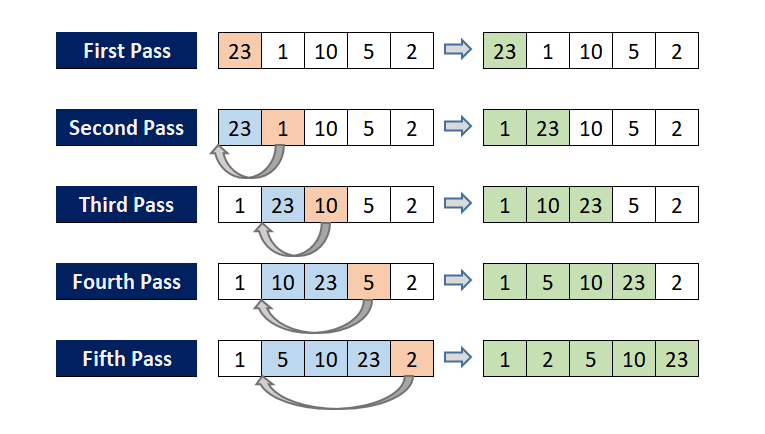
\includegraphics[scale=0.45]{ressources/insert.png}
        \caption{Exemple graphique d’un tri par insertion}
    \label{fig:insert}
\end{figure}
\\
\par
\begin{function}[H]
    \textbf{Variables :}\\
    i,j : entier\;
    tmp,longeur : entier\;
    
    
    \Begin{
        $longeur \leftarrow taille(T)$\;
        \For{$i \leftarrow 1$ \KwTo N-1}{
            $tmp \leftarrow tab[i]$\;
            $j\leftarrow i$\;
                   \While{$j>0$ et $tab[j-1]>tmp$} {
                     $tab[j] \leftarrow tab[j-1]$\;
                     $j \leftarrow j-1$\;
                   } 
            $tab[j] \leftarrow tmp$\;
        }
       
      
    }
    \caption{Insert(Entrée: tab: tableau d'entier; )}
\end{function}


\section{Calcul de complexité}
\subsection{Complexité temporelle}
\par
La complexité d’un algorithme de tri par insertion dépend de la taille n du tableau et de sa nature : si le tableau est déjà trié (ou partiellement trié), la complexité est en effet beaucoup moins important que si le tableau est trié dans l’ordre inverse.
\par
\textbf{Meilleur Cas :}
\par
Ce type de complexité se produit souvent lorsque les éléments du tableau initial sont triés.
 Il faut donc comparer un à un (n-1) éléments.
 \par
* La boucle (pour) s'exécute un nombre de fois égal à N-1.
\par
* la boucle (tant que)  ne s'exécute pas.

\par
Il y a donc N-1 comparaisons et au plus N affectations.
C(n)=N+(N-1)=2N+1.
La complexité du meilleur cas est d'ordre N. Il en résulte une complexité linéaire O(n).

\\
\textbf{Pire Cas :}
\par
Ce type de complexité se produit lorsque les éléments du tableau sont initialement triés dans l’ordre inverse.
\par
A chaque étape, tous les éléments du sous-tableau trié doivent donc être décalés vers la droite pour que l'élément à trier qui est plus petit que tous les éléments déjà triés à chaque étape puisse être placé au  début.
\par
Donc  on effectue l'échange a chaque comparaison.
\par
Le nombre d’échange est alors:
\par
C(n)=2+3+...+N-1= N(N-1)/2 .
\par
La complexité dans le pire des cas est d'ordre N^2. Il en résulte une complexité quadratique  O(n^2).
\par

\textbf{Moyen Cas :}
\par
Ce type de complexité se produit généralement lorsque les éléments d'un tableau sont mélangés de sorte que seulement la moitié des éléments sont décalé, ce qui signifie que chaque élément est plus petit que la moitié des éléments à sa gauche. En considérant un décalage de (p-1)/2 éléments, la complexité moyenne du calcul est donc :
C(n)=1/2+1+...+(N-1)/2= N(N-1)/4

La complexité sera donc la moitié de la complexité du pire cas, mais elle est toujours d'ordre N^{2}, donc c'est une complexité quadratique O(n^{2})


\subsection{Complexité spatiale}
Le tri par insertion englobe une complexité spatiale de O(1) en raison de l'utilisation d'une variable supplémentaire tmp.
\section{Experimentation}
Dans cette partie nous allons voir les résultats des exécutions de cet algorithme sur différents taille de tableau et sur données qui se représentent en 3 configuration ( triée en bon ordre , triée en ordre inverse , aléatoire) 
\subsubsection{Les données du tableau sont triées en bon ordre.}
\\
\begin{tabular}{| c | c | c | c | c | c | c | c | c | c | c |}
    \hline 
     Taille &  10000 & 50000 & 100000 & 500000 & 1000000 & 5000000 & 10000000 & 50000000 \\
    \hline
    temps(s) & 0.000014	& 0.000063 & 0.000136 &	0.000337	& 0.001291 &	0.003248 &	0.012637 &	0.064748	 \\
   \hline
   
\end{tabular}
\par

\subsubsection{Les données du tableau sont triées en ordre inverse.}
\\
\begin{tabular}{| c | c | c | c | c | c | c | c | c | c | c |}
    \hline 
     Taille &  10000 & 50000 & 100000 & 500000 & 1000000 & 5000000 & 10000000 & 50000000 \\
    \hline
    temps(s) & 0.061094 &	1.500352 &	6.068683 	& 101.321114 &	511.278107  &  & & \\
   
   \hline
\end{tabular}
\par
\subsubsection{Les données du tableau sont  positionnés aléatoirement.}
\\
\begin{tabular}{| c | c | c | c | c | c | c | c | c | c | c |}
    \hline 
     Taille &  10000 & 50000 & 100000 & 500000 & 1000000 & 5000000 & 10000000 & 50000000  \\
    \hline
    temps(s) & 0.017770 &	0.537932 & 1.994625	 & 60.600109 &	223.830612 &  & &\\
    \hline
   
   
\end{tabular}
\par
\subsubsection{Le graphe :}
\\
La figure suivante représente les résultats d'exécution de cet algorithme selon les différentes taille du tableau.
\\
\begin{figure}[H]
    \centering
        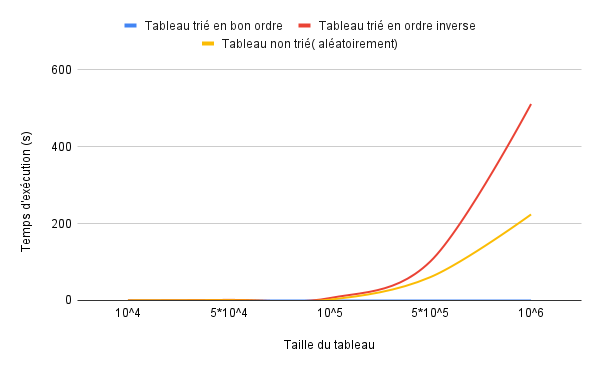
\includegraphics[scale=0.7]{ressources/ChartInsert.png}
        \caption{Temps d'execution du tri par insertion sur les différents taille du tableau }
    \label{fig:insertch}
\end{figure}
\\
D’après le graphique et les tableaux ci-dessus, nous remarquons que le tri par insertion prend beaucoup de temps lors du tri des éléments dans l'ordre inverse ou dans leur positionnement aléatoire, Les courbes s‘évoluent d’une manière quadratique à chaque fois que la taille du tableau augmente. Cependant, si les éléments sont déjà triés, cela fonctionne très bien et ne prend pas beaucoup de temps. 
\par
On en conclut que la complexité théorique est cohérente avec les résultats expérimentaux.

\section{Conclusion}
A partir d'étude expérimentale et théorique de l'algorithme tri par insertion, On constate que malgré sa complexité en temps quadratique sur des données inversées ou triées aléatoirement, il est encore largement utilisé car il est capable de s'exécuter en temps linéaire sur des entrées déjà triées, et de manière très efficace sur de petites entrées.


    
    \newpage
    \onehalfspacing
    \chapter{Tri par Selection}
\section{Fonctionnement de l'algorithme}
Le tri par sélection (ou tri par extraction) est un algorithme de tri par comparaison.
Le principe du tri par selection est de :
\begin{itemize}
  \item rechercher le plus petit élément du tableau, et l'échanger avec l'élément d'indice 0.
  \item rechercher le second plus petit élément du tableau, et l'échanger avec l'élément d'indice 1.
  \item continuer de cette façon jusqu'à ce que le tableau soit entièrement trié.
\end{itemize}
\begin{figure}[H]
    \centering
        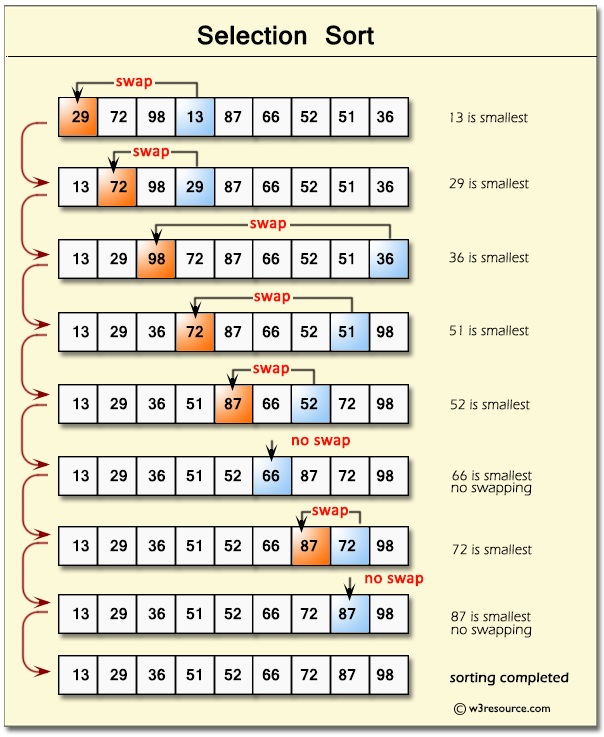
\includegraphics[scale=0.4]{ressources/selection-short.png}
        \caption{Exemple graphique d’un tri par selection}
    \label{fig:fusion}
\end{figure}
\par
Nous pouvons le représenter via le pseudo code suivant :
\par
\begin{function}[H]
    \textbf{Variables :}\\
    i,j : entier\;
    tmp,min : entier\;
    
    
    \Begin{
        \For{$i \leftarrow 1$ \KwTo N-1}{
            $min \leftarrow tab[i]$\;
            $j\leftarrow i$\;
            \For{$j \leftarrow i+1$ \KwTo N-1}{
            \uIf{tab[j] < tab[min]}{
                $min \leftarrow j$\;
               
            }
            }
            $tmp \leftarrow tab[min]$\;
            $tab[min] \leftarrow tab[i]$\;
            $tab[i] \leftarrow tmp$\;
        }
       
      
    }
    \caption{Selection(Entrée: tab: tableau d'entier; )}
\end{function}
\section{Calcul de complexité}
\subsection{Complexité temporelle}
Dans tous les cas, pour trier n éléments, le tri par sélection effectue au plus un nombre linéaire d'échanges :
\par
\textbf{Meilleur Cas:} 
aucun si l'entrée est déjà triée. 
\par
\textbf{Moyenne Cas:}
n-(1/2+...+1/n)= n-nln(n) c'est-à-dire si les éléments sont deux à deux distincts et que toutes leurs permutations sont équiprobables (en effet, l'espérance du nombre d'échanges à l'étape i est 
\par
\textbf{Pire cas:}
n-1 échanges qui est atteint par exemple lorsqu'on trie la séquence 2,3,…,n,1 ;
\par
Et donc le tri par sélection effectue \dfrac{n(n-1)}{2} comparaisons. Et sa complexité est donc O(n^2).
\par
le tableau suivant représente les temps d’exécution théorique en nanoseconde de l’algorithme selon la variation de la taille de l’expression :
\small
\begin{center}
\begin{tabular}{| c | c | c | c | c | c | c | c | c | c | c | c | c |}
    \hline
    N &  10 & 50 & 100 & 500 & 1000 & 5000 & 10000 & 100000 & 1000000 & 10000000 \\
    \hline
    t(ns) & 45 &
1225&
4950&
124750&
499500&
12497500&
49995000&
499995*10^4&
4999995*10^5&
49999995*10^6 \\
    \hline
\end{tabular}  
\end{center}
\par
La figure suivante représente l’évolution du temps d’exécution selon la longueur du tableau: 
\begin{figure}[H]
    \centering
        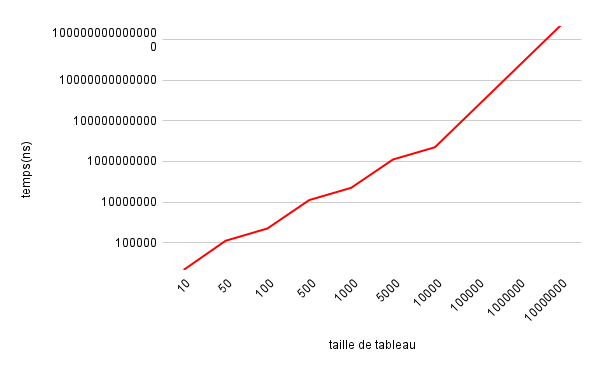
\includegraphics[scale=0.7]{ressources/chartselecttheorique.png}
        \caption{Temps d'exécution théorique du Tri Selection selon la longueur du tableau}
    \label{fig:temps_exec_selec_theo}
\end{figure} 
\subsection{Complexité spatiale}
Dans tous les cas O(1)
\section{Experimentation}
Le tableau suivant représente les temps d’exécution en nanoseconde de l’algorithme selon la variation de la taille et la configuration de l'entree .
\subsubsection{Les données du tableau sont triées en ordre inverse.}
\small
\begin{center}
\resizebox{19cm}{!}{
\begin{tabular}{| c | c | c | c | c | c | c | c | c | c | c |}
    \hline
    N &  10000 & 50000 & 100000 & 500000 & 1000000 & 5000000 & 10000000 & 50000000 \\
    \hline
    Temp(s) & 0.038229&
1.092237&
3.880469&
89.18019&
//&
//&//&//  \\
    \hline
\end{tabular}}
\end{center}
\normalsize
\subsubsection{Les données du tableau sont triées en bon ordre.}
\small
\begin{center}
\resizebox{19cm}{!}{
\begin{tabular}{| c | c | c | c | c | c | c | c | c | c | c |}
    \hline
    N &  10000 & 50000 & 100000 & 500000 & 1000000 & 5000000 & 10000000 & 50000000 \\
    \hline
    Temp(s) & 0.0324&
0.6452&
2.94&
78.785&//&//&
//&
//  \\
    \hline
\end{tabular}}
\end{center}
\normalsize
\par
\subsubsection{Les données du tableau sont aleatoires.}
\small
\begin{center}
\resizebox{19cm}{!}{
\begin{tabular}{| c | c | c | c | c | c | c | c | c | c | c |}
    \hline
    N &  10000 & 50000 & 100000 & 500000 & 1000000 & 5000000 & 10000000 & 50000000 \\
    \hline
    Temp(s) & 0.026639&
0.639662&
3.268848&
75.4&
//&
//&
//&
//  \\
    \hline
\end{tabular}}
\end{center}
\normalsize
\par
La figure suivante représente l’évolution du temps d’exécution en (s) selon la taille et la configuration du tableau :
\begin{figure}[H]
    \centering
        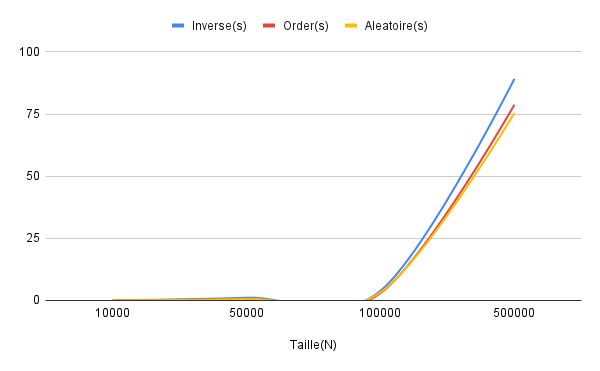
\includegraphics[scale=0.7]{ressources/selectexp.png}
        \caption{Temps d'exécution du programme selon la taille du tableau}
    \label{fig:temps_exec_dico_theo}
\end{figure} 
\par
Depuis le graphe, on observe que le temps d’exécution évolue de manière quadratique avec l’augmentation de la taille du tableau quelque soit la configuration utilise, ce qui correspond bien à la complexité théorique calculée auparavant.
\section{Conclusion}
L’algorithme de tri par selection se caractérise par son fonctionnement inconditionnel sur n’importe quel tableau. Par ailleurs, elle est coûteuse en temps. 
    
    \newpage
    \onehalfspacing
    \chapter{Tri rapide}
\section {Description}
Le tri rapide, aussi appelé "tri de Hoare" du nom de son inventeur "Tony Hoare" ou "Quick Sort" en anglais, est considéré comme l'algorithme le plus performant des tris en table qui est certainement celui qui est le plus employé dans les programmes depuis son invention en 1960. Cette méthode illustre le principe dit « diviser pour régner », qui consiste à appliquer récursivement une méthode destinée à un problème de taille donnée à des sous-problèmes similaires, mais de taille inférieure. Ce principe général produit des algorithmes qui permettent souvent d’importantes réductions de complexité

\section{Fonctionnement de l'algorithme}
Le principe de ce tri est d’ordonner le vecteur T[n] en cherchant dans celui-ci une clé pivot autour de laquelle réorganiser ses éléments. Donc On considère un élément au hasard dans le tableau, le pivot et on procède à une partition du tableau en 2 zones : les éléments inférieurs ou égaux au pivot dans un coté et les éléments supérieurs ou égaux au pivot
dans l'autre coté pui on place le pivot dans sa position appropriée. On répète récursivement la procédure sur chacune des partitions créées en considérant un pivot dans chaque partie jusqu’à ce qu’elle soit réduite à une liste à un seul élément. [3]
\begin{figure} [H]
        \centering
        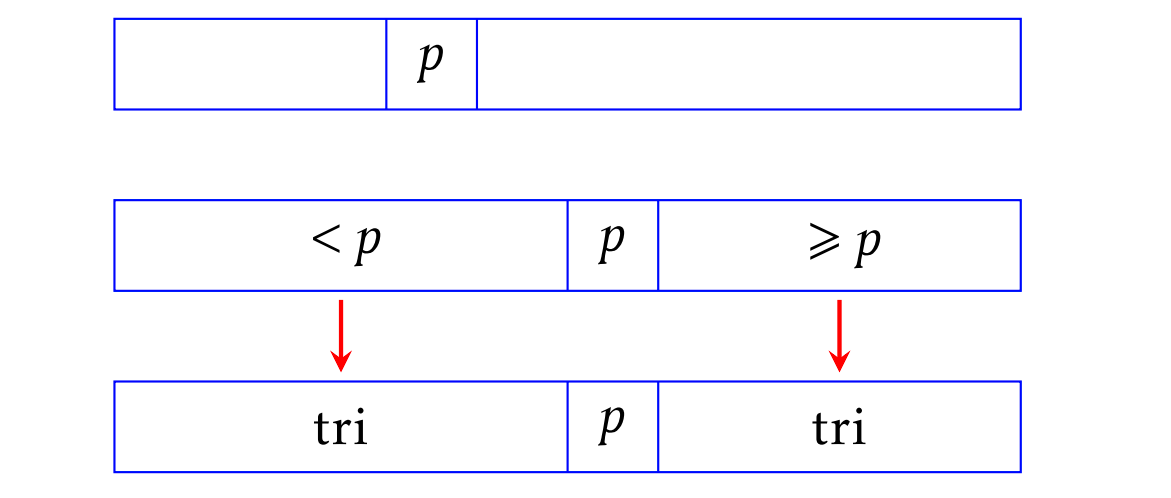
\includegraphics[scale=0.4]{ressources/tri_rapide.PNG}
        \caption{Illustration Tri Rapide }
        \label{fig:rapide}
     \end{figure}
Ils existent plusieurs methodes de choix du pivot qui est determinant pour la performance de l'algorithme:
\begin{enumerate}
    \item Le pivot est le premier élément du tableau
    \item Le pivot est le dernier élément du tableau
    \item Le pivot est au millieu du tableau
    \item Le pivot est choisi au hasard
    \item pivot est trouvé en recherchant la médiane
\end{enumerate}
Dans ce TP nous avons testé les trois premières méthodes comme il est demandé dans l'énoncé.\\
Pour programmer le Tri Rapide nous allons utiliser deux procédures:
\begin{enumerate}
    \item Partition:une fonction qui divise un tableau en entrée en deux sous listes et retourne le pivot. Il peut y avoir plusieurs façons de faire la partition, dans le cas de la première et la deuxième methodes  on commençe le parcours du tableau par l'élément le plus à gauche ou à droite selon le pivot choisi et on utilise un compteur p qui garde la trace de l'indice des éléments plus grands que le pivot. Pendant le parcours, si on trouves un élément plus petit que le pivot, on incrémente p et l'élément actuel sera échangé avec Tab[p]. Sinon il sera ignoré.
    Dans la troisième méthode on parcourt le tableaux à partir des deux extrémités, jusqu'à rencontrer un élément supérieur au pivot dans la prtie droite du tableau ou le contraire dans la pertie gauche et on permute entre les deux.
\end{enumerate}
Partition  ainsi que la procédure TriRapide qui assure l'application du 
même processus sur les sous listes droites et gauches générées (assure la récursivité).\\
\subsection{Méthode 1 : Le pivot est le premier élément du tableau }
\par
\begin{function}[H]
    \textbf{Variables :}\\
     i : entier\;
     p,pivot : entier\;
    \Begin{
        $p \leftarrow deb$\;
        $pivot \leftarrow tab[deb]$\;
        \For{$i \leftarrow deb+1$ \KwTo fin$}{
            \If {tab[i]$<pivot$} {
                p++ \;
                permuter(tab[i]$,p$);
            }
        }
        permuter(tab[p]$,deb$)\;
        \textbf {retourner} p;
      
    }
    \caption{Partition1(Entrée: tab: tableau d'entier, deb:entier, fin:entier)}
\end{function}

\par
\begin{function}[H]
    \textbf{Variables :}\\
     pivot : entier\;
    \Begin{
            \If {deb$<fin$} {
                pivot$ \leftarrow Partition1(tab$,deb$,fin$) \;
                TriRapide1$(tab$, deb$, pivot-1$) \;
                TriRapide1$(tab$, pivot+1$,fin$) \;
                
            }
         }
    \caption{TriRapide1(Entrée: tab: tableau d'entier, deb:entier, fin:entier)}
\end{function}

\subsection{Méthode 2 : Le pivot est le dernier élément du tableau}
\par
\begin{function}[H]
    \textbf{Variables :}\\
     i : entier\;
     p,pivot : entier\;
    \Begin{
        $p \leftarrow fin$\;
        $pivot \leftarrow tab[fin]$\;
        \For{$i \leftarrow fin-1$ \KwTo deb$}{
            \If {tab[i]$ > pivot$} {
                p-- \;
                permuter(tab[i]$,p$);
            }
        }
        permuter(tab[p]$,fin$)\;
        \textbf {retourner} p \;
      
    }
    \caption{Partition2(Entrée: tab: tableau d'entier, deb:entier, fin:entier)}
\end{function}
\par
\begin{function}[H]
    \textbf{Variables :}\\
     pivot : entier\;
    \Begin{
            \If {deb$<fin$} {
                pivot$ \leftarrow Partition2(tab$,deb$,fin$) \;
                TriRapide2$(tab$, deb$, pivot-1$) \;
                TriRapide2$(tab$, pivot+1$,fin$) \;
                
            }
         }
    \caption{TriRapide2(Entrée: tab: tableau d'entier, deb:entier, fin:entier)}
\end{function}
\subsection{Méthode 3 : Le pivot est au millieu du tableau}
\par
\begin{function}[H]
    \textbf{Variables :}\\
     i,j,x: entier\;
     pivot: entier\;
    \Begin{
        $x \leftarrow (fin$-deb$)/2$ \;
        $pivot \leftarrow $tab[x] \;
        $i \leftarrow deb-1$ \;
        $j\leftarrow fin$\;
        \While {i<=j}
        {
           \While {$tab[i]<pivot$;} {$i \leftarrow $i+1 ;}
           \While  {$tab[j]>pivot$;} {$j \leftarrow $j+1 ;}
           \If{i$<=j$}{$Permuter($tab,$i,$j);}
           }
        
    \textbf{retourner} $i\;\\
     }
    \caption{Partition3(Entrée: tab: tableau d'entier, deb:entier, fin:entier)}
\end{function}

\par
\begin{function}[H]
    \textbf{Variables :}\\
     pivot : entier\;
    \Begin{
            \If {deb$<fin$} {
                pivot$ \leftarrow Partition3(tab$,deb$,fin$) \;
                TriRapide3$(tab$, deb$, pivot-1$) \;
                TriRapide3$(tab$, pivot+1$,fin$) \;
                
            }
         }
    \caption{TriRapide3(Entrée: tab: tableau d'entier, deb:entier, fin:entier)}
\end{function}
\section{Calcul de complexité}
\subsection{Complexité temporelle}
Pour calculer la complexité des algorithmes récursives de Tri Rapide nous utilisons la formule suivante : \\
le nombre des niveaux de partition * temps nécessaire pour un niveau

sachant que la complexité temporelle pour réaliser la partition  est de l'ordre O(n) car à chaque niveau de partitionnement,un total de n éléments sera divisé en partitions gauche et droite (1 × n au premier niveau, 2 × n/2 au deuxième, 4 × n/4 au troisième, etc.) L'effort total est donc le même à tous les niveaux de partitionnement.\\


   \begin{enumerate}
    \item Meilleur cas: le meilleur ca s'achève lorsque le tableau Tab de taille n se divise sur 2 partie égales de n/2 éléments et les sous tableaux a leurs tour se divisent en deux sous-listes de même taille.
      \begin{figure} [H]
        \centering
        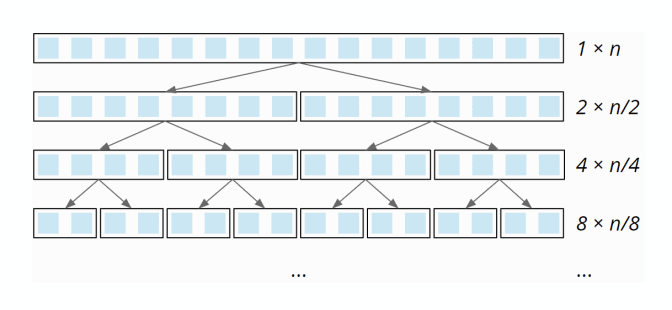
\includegraphics[scale=0.45]{ressources/Quicksort_best_case_time_complexity.png}
        \caption{Tri Rapide complexité meilleur cas }
        \label{fig:rapide}
     \end{figure}
     
    Le nombre des niveaux de partition:
    \[
   \frac{n}{2^k}=1
   \]
    \[
   n=2^k
   \]
    \[
   \log_2 n = k \log_2 2
   \]
  \[
   k= \log_2 n
  \]
  Donc Dans le meilleur des cas, la complexité temporelle est : O(n * log n)\\
  Cette complexité est atteinte dans le cas suivant:\\
    *le pivot choisi est le premier élément dans le tableau ou le dernier et les éléments sont aléatoires.\\
    * le pivot choisi est toujours au millieu du tableau
     
   \item Pire cas: le pire cas correspond au cas où le tableau ne serait pas divisé en deux partitions de tailles approximativement égales, mais une de longueur 0 et une de longueur n-1 (tous les éléments sauf l'élément pivot) alors l'effort de partitionnement décroît linéairement de n à 0 avec la liste droite ou gauche vide selon le pivot choisi.
   Ainsi nous calculons la comlexité comme suit: 
   \[
   n+n-2+n-3+n-4...+2 =\frac{n(n+1)}{2}-1 \\
   = n^2 + n \\
   = O(n^2) \\
   \]
   \begin{figure} [H]
       \centering
       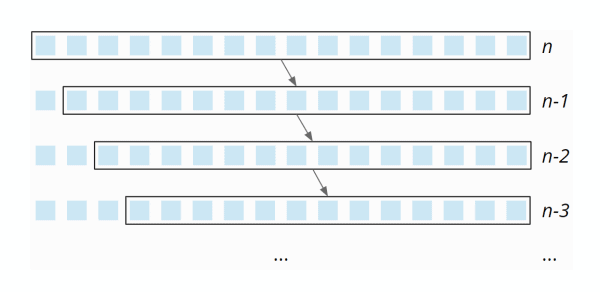
\includegraphics[scale=0.45]{ressources/Quicksort_worst_case_time_complexity-600x292.png}
       \caption{Tri Rapide complexité pire cas}
       \label{fig:rapidel}
   \end{figure}
    Cette complexité est atteinte lorsque le pivot choisi est a la tête ou a la fin du tableau et ce dernier est triée d'une manière descendante ou ascendante.
   \item Moyen cas: est atteint lorsque le tableau serait divisé successivement
en deux sous-listes de taille à peu près équivalente par exemple n/10 et 9n/10.
En utilisons la formule au dessus nous aboutissons à une complexité similaire au meilleur cas O(n * log n).
\end{enumerate}

  


\subsection{Complexité spatiale}
La complexité spatiale de Tri Rapide est dans tout les cas O(log n)
car pour chaque niveau de récursion, nous avons besoin de mémoire supplémentaire sur la pile. Come nous avons vu quand nous avons calculé la complexité temporelle dans le cas moyen et le meilleur cas, la profondeur maximale de récursion est limitée par O(log n) .
Dans le pire des cas, la profondeur maximale de récursion est de n
\section{Experimentation}
Dans cette partie nous allons voir les résultats des exécutions des trois méthodes de l'algorithme de Tri Rapide sur différentes taille de tableau qui se représentent en 3 configuration ( triée en bon ordre , triée en ordre inverse , aléatoire) 
\subsection{Les données de tableau sont triées en bon ordre}

 \begin{figure}[H]
    \centering
        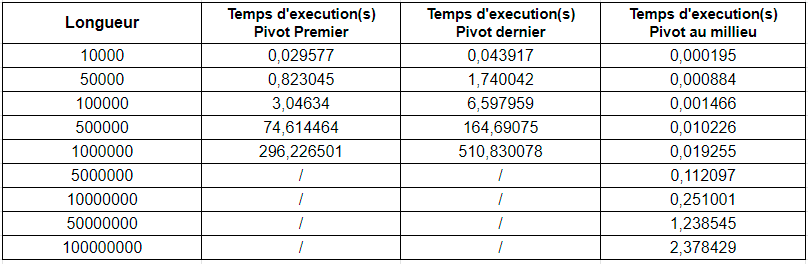
\includegraphics[scale=0.7]{ressources/trieeT.PNG}
        \caption{Tableau représentant le temps d'execution en s des trois méthodes de tri rapide selon les différentes tailles des données d'entrée triées en bon ordre}
    \label{fig:fusion}
\end{figure}
\par
 \begin{figure}[H]
    \centering
        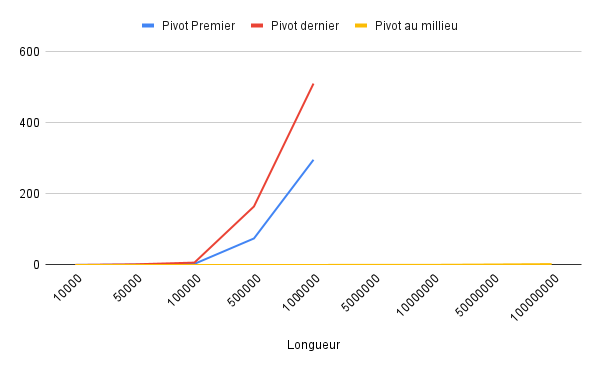
\includegraphics[scale=0.7]{ressources/triee.png}
        \caption{graphique représentant le temps d'execution en s des trois méthodes de tri rapide selon les différentes tailles de tableau}
    \label{fig:fusion}
\end{figure}


\subsection{Les données de tableau sont triées en ordre inverse }
\begin{figure}[H]
    \centering
        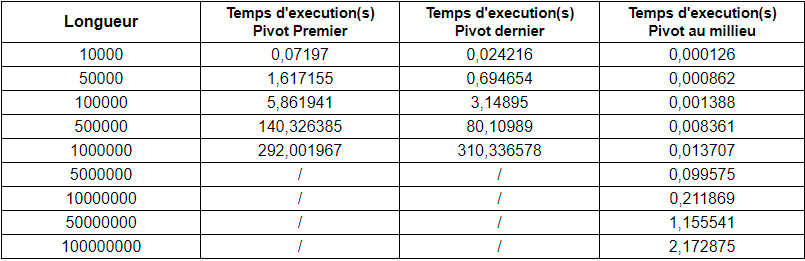
\includegraphics[scale=0.7]{ressources/invT.PNG}
        \caption{Tableau représentant le temps d'execution en s des trois méthodes de tri rapide selon les différentes tailles des données d'entrée triées en ordre inverse}
    \label{fig:fusion}
\end{figure}

\begin{figure}[H]
    \centering
        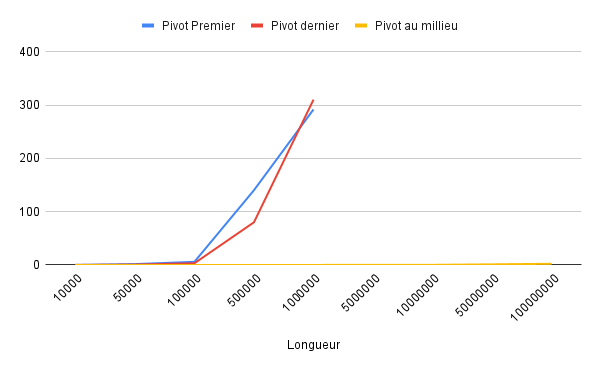
\includegraphics[scale=0.7]{ressources/inv.png}
        \caption{graphique représentant le temps d'execution en s des trois méthodes de tri rapide selon les différentes tailles de tableau}
    \label{fig:fusion}
\end{figure}

\subsection{Les données de tableau sont positionnés aléatoirement}
\begin{figure}[H]
    \centering
        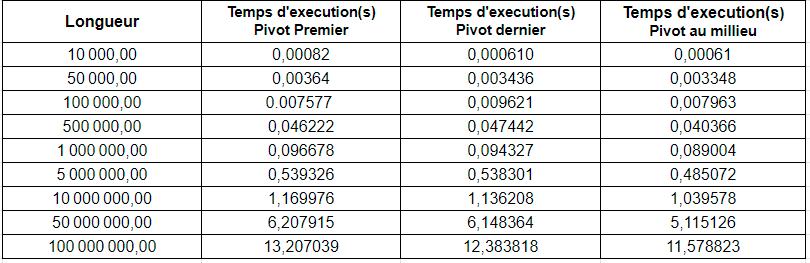
\includegraphics[scale=0.7]{ressources/randT.PNG}
        \caption{Tableau représentant le temps d'execution en s des trois méthodes de tri rapide selon les différentes tailles des données d'entrée sont aléatoires}
    \label{fig:fusion}
\end{figure}

\begin{figure}[H]
    \centering
        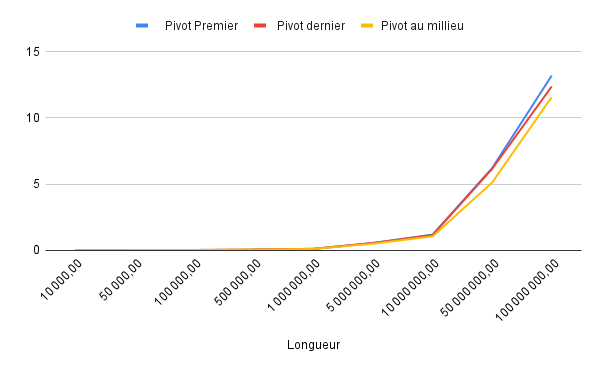
\includegraphics[scale=0.7]{ressources/random.png}
        \caption{graphique représentant le temps d'execution en s des trois méthodes de tri rapide selon les différentes tailles de tableau}
    \label{fig:fusion}
\end{figure}
\section{Analyses Des Résultats}
\paragraph{Cas Pivot au début:} \\
Pour des données d'entrée distribuées de manière aléatoire, le temps nécessaire est légèrement supérieur au double si la taille du tableau est doublée. Cela correspond au temps d'exécution quasi-linéaire attendu O(n log n).\\
Pour les données d'entrée triées dans l'ordre croissant ou décroissant, le temps requis quadruple lorsque la taille de l'entrée est doublée, nous avons donc un temps quadratique O(n²).\\
Le tri des données dans l'ordre décroissant ne prend qu'un peu plus de temps que le tri des données dans l'ordre croissant et l'execution s'arrete si la taille de tableau dépasse 10^6.
\paragraph{Cas Pivot au dérnier:} 
Dans ce cas de choix de pivot les résultas sont approximativement similaires aux ceux de choix de pivot au début: une complexité O(n log n) pour des données de tableau  aléatoires et O(n²) si les données sont triées avec une légère amélioration sur les tableaux triées dans l'ordre décroissant.\\
\paragraph{cas Pivot au millieu :}
Pour des données d'entrée triées et non triées l'étude de l'évolution de temps d'execution correspond au temps d'exécution quasi-linéaire attendu O(n log n).\\
L'algorithme est nettement plus rapide pour les données d'entrée prétriées que pour les données aléatoires.\\

\section{Conclusion}
Le Tri rapide est l’algorithme de tri le plus utilisé en raison de sa complexité temporelle optimale en moyenne de O(n log n) et sa complexité spatiale O(log n) ce qui en fait un excellent choix pour les situations où l'espace est limité. 
Bien qu'il offre ces avantages il est considéré comme instable à cause des permutations des éléments et très improbable avec choix du pivot qui affecte considérablement sa complexité où elle atteint O(n^2)$ dans les pires cas mais il reste le meilleur choix partout où la stabilité n'est pas nécessaire.

    
    
    \newpage
    \onehalfspacing
    \chapter{Tri par fusion}
\section{Description de l’objectif de l’algorithme}
En informatique, un tableau est une structure de données représentant une séquence finie d’éléments définis par un index représentant leurs positions au sein du tableau. 
C’est un type de conteneur que l’on retrouve dans un grand nombre de langages de programmation et est l’un des plus utilisés dû à sa simplicité. Les données du tableau étant accessible individuellement il est nécessaire de faire une recherche lorsque l’on souhaite accéder a une valeur spécifique du tableau. Cependant, lorsque la taille de la structure est grande il devient difficile d’y accéder efficacement.
\section{Fonctionnement de l'algorithme}
Le tri par fusion aussi appeler tri dichotomique est un exemple classique d’algorithme de division pour régner. 
L’opération principale de l’algorithme est la fusion, qui consiste à réunir deux listes triées en une seule. L’efficacité de l’algorithme vient du fait que deux listes triées peuvent être fusionnées en temps linéaire . On peut résumer son fonctionnement en deux étapes :
\par
\begin{enumerate}
  \item Divisez la liste non triée en sous-listes jusqu'à ce qu'il y ait N sous-listes avec un élément dans chacune (N est le nombre d'éléments dans la liste non triée).
  \item Fusionnez les sous-listes deux à la fois pour produire une sous-liste triée, répétez cette opération jusqu'à ce que tous les éléments soient inclus dans une seule liste.
\end{enumerate}

\begin{figure}[H]
    \centering
        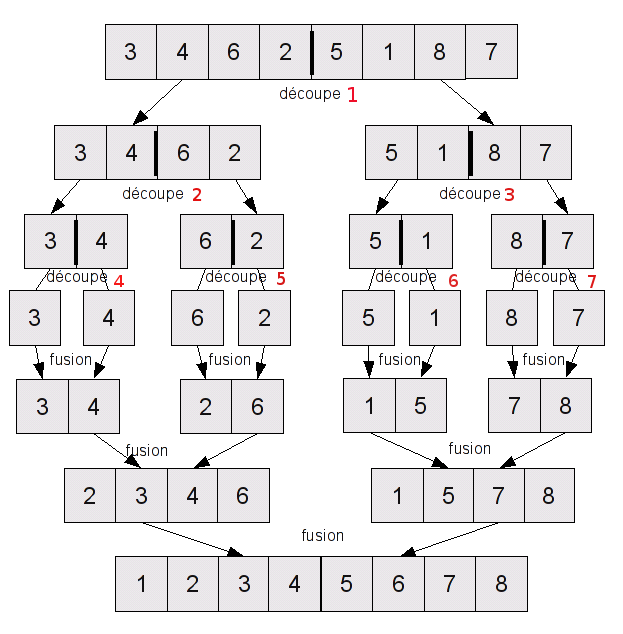
\includegraphics[scale=0.7]{ressources/fusion.png}
        \caption{Exemple graphique d’un tri par fusion}
    \label{fig:fusion}
\end{figure}
\par
Afin d’optimiser le déroulement du tri, nous utilisons 2 fonctions distinctes. Une fonction TriFusion qui divise le tableau récursivement et une fonction Fusion qui elle trie les sous tableaux
avant de les fusionner à nouveau. Nous pouvons le représenter via le pseudo code suivant :
\par
\begin{function}[H]
    \textbf{Variables :}\\
    TabG, TabD : tableau d'entier\;
    SousTab1, SousTab2, SousTab1Index, SousTab2Index, SousTabFusionIndex : entier\;
    \Begin{
        $milieu \leftarrow \frac{droite + gauche}{2}$\;
        $SousTab1  \leftarrow milieu - gauche + 1$\;
        $SousTab2  \leftarrow droite - milieu$\;
        \For{$i \leftarrow 1$ \KwTo $SousTab1$}{
            $tabG[i] \leftarrow tab[gauche + i]$\;
        }
        \For{$j \leftarrow 1$ \KwTo $SousTab2$}{
            $tabG[j] \leftarrow tab[mid + 1 + j]$\;
        }
        $SousTab1  \leftarrow 0$\;
        $SousTab2  \leftarrow 0$\;
        $SousTabFusionIndex  \leftarrow gauche$\;
        \While{$SousTab1Index < SousTab1$ et $SousTab2Index < SousTab2$}
       {
            %\\
            \uIf{tabG[SousTab1Index] <= tabD[SousTab2Index]}{
                $tab[SousTabFusionIndex] \leftarrow tabG[SousTab2Index]$\;
                $SousTab1Index++$\;
            }
            \Else {
                $tab[SousTabFusionIndex] \leftarrow tabD[SousTab2Index]$\;
                $SousTab2Index++$\;
            }
            $SousTabFusionIndex++$\;
        %\EndWhile
        }
        \While{$SousTab1Index < SousTab1$}
       {
            %\\
            $tab[SousTabFusionIndex] \leftarrow tabG[SousTab1Index]$\;
            $SousTab1Index++$\;
            $SousTabFusionIndex++$\;
        %\EndWhile
        }
        \While{$SousTab2Index < SousTab2$}
       {
            %\\
            $tab[SousTabFusionIndex] \leftarrow tabG[SousTab2Index]$\;
            $SousTab1Index++$\;
            $SousTabFusionIndex++$\;
        %\EndWhile
        }
    }
    \caption{Fusion(Entrée: tab: tableau d'entier; droite, gauche: entier;)}
\end{function}

\begin{function}[H]
    \textbf{Variables :}\\
    milieu : entier\;
    \Begin{
        \tcp{On divise le tableau en 2 de manière recursive puis on les tri avant de les fusionner}
        \If{$debut >= fin$}
            {retour\;}
        \tcp{On calcule l'index du milieu du tableau}
        $milieu \leftarrow debut + (fin - debut) / 2$\;
        TriFusion(tab, debut, milieu)\;
        TriFusion(tab, milieu + 1, fin)\;
        \tcp{On utilise la fonction fusion pour trier puis fusioner les sous tableaux en un seul tableau trié}
        Fusion(tab, debut, mid, fin)\;
    }
    \caption{TriFusion(Entrée: tab: tableau d'entier; debut, fin: entier;)}
\end{function}

\section{Calcul de complexité}

\subsection{Complexité temporelle}
la fonction merge consiste a decouper une liste de taille N en N sous-listes avec un élément dans chacune donc on doit parcourir tout le tableau qui est donc de complexite O(n). 
\subsubsection{Complexité d'une fonction récursive}
Pour calculer la complexité d'une fonction récursive, il faut souvent utiliser une formule de récurrence. 
apres la division , on aura deux problemes a résoudre de taille N/2.
On les résout récursivement 
on exprime donc la complexité au pire cas de merge sort par n(log n + 1) 
quelque soit l'order des elements de tableau , le tri fusion consiste toujour a le decouper en sous listes jusqu'a ce qu'il ya que des feuilles et les fusionner .
\textbf{et donc La complexité de tri par fusion est toujours( meilleur , moyenne et pire cas) égale à : O(nln(n)).}
\\
\par
le tableau suivant représente les temps d’exécution théorique en nanoseconde de l’algorithme selon la variation de la taille de l’expression :
\small
\begin{center}
\begin{tabular}{| c | c | c | c | c | c | c | c | c | c | c | c | c |}
    \hline
    N &  10 & 50 & 100 & 500 & 1000 & 5000 & 10000 & 100000 & 1000000 & 10000000 \\
    \hline
    t(ns) & 10 &
84.95&
200&
1349.48&
3000&
18494.85&
40000&
500000&
6000000&
70000000 \\
    \hline
\end{tabular}  
\end{center}
\par
La figure suivante représente l’évolution du temps d’exécution selon la longueur du tableau: 
\begin{figure}[H]
    \centering
        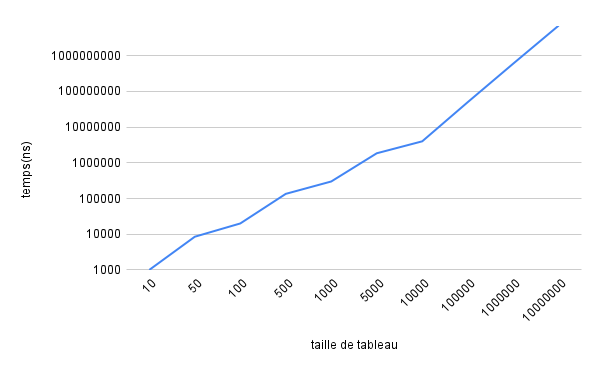
\includegraphics[scale=0.7]{ressources/chartfusiontheorique.png}
        \caption{Temps d'exécution théorique du programme selon la longueur du tableau}
    \label{fig:temps_exec_dico_theo}
\end{figure} 
\subsection{Complexité spatiale}
la complexite spatiale de tri fusion est O(n).
\section{Experimentation}
Le tableau suivant représente les temps d’exécution en nanoseconde de l’algorithme selon la variation de la taille et la configuration de l'entree .
\subsubsection{Les données du tableau sont triées en ordre inverse.}
\small
\begin{center}
\resizebox{19cm}{!}{
\begin{tabular}{| c | c | c | c | c | c | c | c | c | c | c |}
    \hline
    N &  10000 & 50000 & 100000 & 500000 & 1000000 & 5000000 & 10000000 & 50000000 \\
    \hline
    t1(s) & 0.00042 &	0.002448 &	0.00494 &	0.025386 &	0.055339&	0.304839 & 0.603316&	3.768904 \\
    \hline
    t2(s) & 0.000808 &	0.004676 &	0.009942&	0.052479&	0.113005&	0.624881 & 1.28433&	7.613348  \\
    \hline
    t3(s) & 0.001207 &	0.00691	&0.014647&	0.081096&	0.169904&	0.944664 & 1.942545	&11.444372  \\
    \hline
    t4(s) & 0.001619&	0.009289&	0.019483&	0.10869&	0.227738&	1.259653 & 2.613055&	15.351673  \\
    \hline
    t5(s) & 0.001993&	0.011645&	0.024382&	0.133484&	0.284621&	1.568324 & 3.303382	&19.305843  \\
    \hline
    t6(s) & 0.00238	&0.013891&	0.029357&	0.160016&	0.342119&	1.905382 & 3.922201&	23.20739  \\
    \hline
    t7(s) & 0.002792&	0.016027&	0.034042&	0.186831&	0.400959&	2.220602 & 4.579432&	27.165472  \\
    \hline
    t8(s) & 0.003176&	0.017979&	0.038603&	0.213543&	0.459195&	2.531605 & 5.232867	&31.079348 \\
    \hline
    t9(s) & 0.003569&	0.020067&	0.043068&	0.241344&	0.512189&	2.844363 & 5.811679&	34.919087 \\
    \hline
    t10(s) & 0.003952&	0.022506&	0.047414&	0.268108&	0.569763&	3.172519 & 6.390016	&38.880528  \\
    \hline
    Moyenne(s) & 0.002192&	0.012544&	0.026588&	0.147098&	0.313483&	1.737683 & 3.568282	&21.273597  \\
    \hline
\end{tabular}}
\end{center}
\normalsize
\subsubsection{Les données du tableau sont triées en bon ordre.}
\small
\begin{center}
\resizebox{19cm}{!}{
\begin{tabular}{| c | c | c | c | c | c | c | c | c | c | c |}
    \hline
    N &  10000 & 50000 & 100000 & 500000 & 1000000 & 5000000 & 10000000 & 50000000 \\
    \hline
    t1(s) & 0.000569&	0.002628&	0.005863&	0.030151&	0.061241&	0.360749&	0.709762	&4.124928 \\
    \hline
    t2(s) & 0.001068&	0.005192&	0.011261&	0.059449&	0.121092&	0.682264&	1.400675&	8.280286  \\
    \hline
    t3(s) & 0.001561&	0.007656&	0.016423&	0.088011&	0.176175&	1.001632&	2.058852&	12.254911  \\
    \hline
    t4(s) & 0.00202	&0.010261&	0.021879&	0.11565&	0.228058&	1.310229&	2.746449&	15.998439  \\
    \hline
    t5(s) & 0.002476&	0.012919&	0.027025&	0.144914&	0.283809&	1.661196&	3.447879&	19.919397  \\
    \hline
    t6(s) & 0.002887&	0.015353&	0.032353&	0.1737&	0.341154&	2.013703&	4.154876&	23.882657  \\
    \hline
    t7(s) & 0.003342&	0.017781&	0.037866&	0.202648&	0.398567&	2.376409&	4.836434&	27.617182  \\
    \hline
    t8(s) & 0.003832&	0.02029&	0.043166&	0.232642&	0.459596&	2.74455&	5.524018&	31.593124 \\
    \hline
    t9(s) & 0.004247&	0.022741&	0.048409&	0.262612&	0.511865&	3.105877&	6.199981&	35.648717 \\
    \hline
    t10(s) & 0.004753&	0.025202&	0.053627&	0.292089&	0.564445&	3.421129&	6.906015&	39.616554  \\
    \hline
    Moyenne(s) & 0.002675&	0.014002&	0.029787&	0.160187&	0.3146&	1.867774&	3.798494&	21.89362  \\
    \hline
\end{tabular}}
\end{center}
\normalsize
\par
\subsubsection{Les données du tableau sont aleatoires.}
\small
\begin{center}
\resizebox{19cm}{!}{
\begin{tabular}{| c | c | c | c | c | c | c | c | c | c | c |}
    \hline
    N &  10000 & 50000 & 100000 & 500000 & 1000000 & 5000000 & 10000000 & 50000000 \\
    \hline
    t1(s) & 0.000659&	0.003734&	0.007724&	0.044176&	0.082721&	0.449917&	1.040069&	5.768796 \\
    \hline
    t2(s) & 0.001049&	0.006208&	0.012345&	0.074345&	0.140179&	0.734552&	1.777799&	9.790986  \\
    \hline
    t3(s) & 0.001447&	0.00852&	0.01707&	0.103247&	0.197034&	1.049007&	2.509943&	13.84349  \\
    \hline
    t4(s) & 0.001784&	0.011054&	0.02166&	0.132922&	0.252066&	1.37088&	3.239306&	17.834287  \\
    \hline
    t5(s) & 0.002294&	0.013381&	0.026351&	0.16232&	0.307356&	1.704408&	3.973541&	21.750978  \\
    \hline
    t6(s) & 0.002644&	0.015765&	0.030871&	0.192797&	0.365797&	2.039695&	4.707078&	25.682164  \\
    \hline
    t7(s) & 0.00303&	0.018165&	0.035004&	0.222074&	0.420898&	2.385981&	5.453311&	29.653989 \\
    \hline
    t8(s) & 0.003439&	0.020634&	0.039404&	0.249832&	0.480518&	2.729575&	6.194547&	33.541621 \\
    \hline
    t9(s) & 0.003828&	0.022892&	0.043711&	0.278123&	0.542099&	3.078519&	6.927452&	37.484699 \\
    \hline
    t10(s) & 0.004228&	0.02522&	0.048058&	0.307679&	0.596437&	3.417302&	7.677789&	41.405992  \\
    \hline
    Moyenne(s) & 0.00244&	0.014557&	0.02822&	0.176752&	0.338511&	1.895984&	4.350083&	23.6757  \\
    \hline
\end{tabular}}
\end{center}
\normalsize
\par
La figure suivante représente l’évolution du temps d’exécution en (s) selon la taille et la configuration du tableau :
\begin{figure}[H]
    \centering
        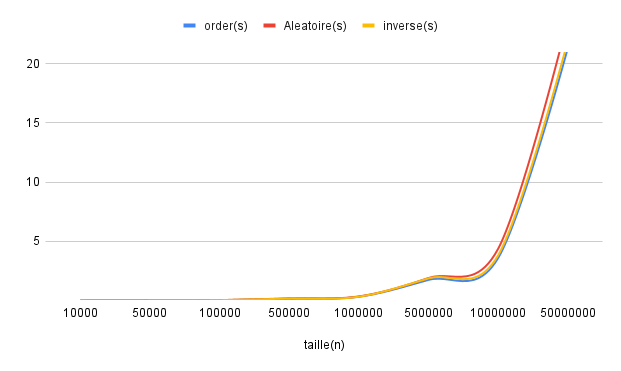
\includegraphics[scale=0.7]{ressources/chartfusion.png}
        \caption{Temps d'exécution du programme selon la taille du tableau}
    \label{fig:temps_exec_dico_theo}
\end{figure} 
\par
Depuis les graphes, on observe que le temps d’exécution évolue de manière linéairethemtique avec l’augmentation de la taille du tableau quelque soit l'ordre, ce qui correspond bien à la complexité théorique calculée auparavant.

\par
\section{Conclusion}
D'apres l'etude theorique et experimentale de la fonction tri fusion on observe que le temps d'execution evolue de maniere lineairethemtique avec l'augmentation de la taille du tableau quelque soit la configuration utilisee , O(nlog(n)) est pratiquement une complexite optimale pour les configuration inverse et aleatoire mais il y'a meilleur fonctions de tri avec une complexite plus optimale lorsque on parle de la configuration en bon ordre.

    
    \newpage
    \onehalfspacing
    \chapter{Tri par bulle}
\section{Fonctionnement de l'algorithme}
Le tri à bulles ou tri par propagation1 est un algorithme de tri. Il consiste à comparer répétitivement les éléments consécutifs d'un tableau, et à les permuter lorsqu'ils sont mal triés.
\par
Le principe du tri à bulles (bubble sort ou sinking sort) est de comparer deux à deux les éléments x1 et x2 consécutifs d'un tableau et d'effecteur une permutation si x1 > x2. On continue de trier jusqu'à ce qu'il n'y ait plus de permutation.
\begin{figure}[H]
    \centering
        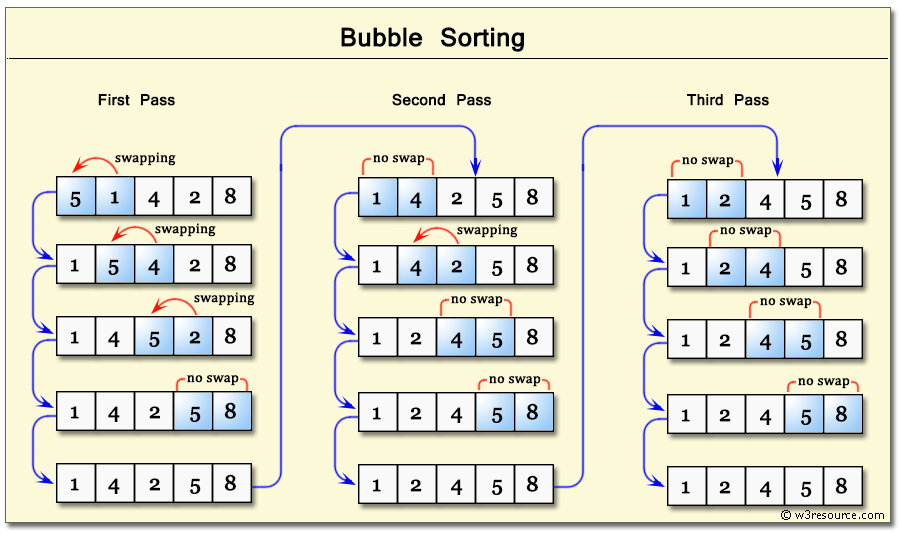
\includegraphics[scale=0.5]{ressources/bubble-sort.png}
        \caption{Exemple graphique d’un tri par bulle}
    \label{fig:fusion}
\end{figure}
\par
Nous pouvons le représenter via le pseudo code suivant :
\par
\begin{function}[H]
    \textbf{Variables :}\\
    i,j : entier\;
    tmp,b : entier\;
    
    
    \Begin{
        \For{$i \leftarrow 1$ \KwTo N-1}{
            $b \leftarrow true$\;
            \While{b} {
            \For{$j \leftarrow i+1$ \KwTo N-1}{
            
            \uIf{tab[j] > tab[j+1]}{
            $b \leftarrow false$\;
                $tmp \leftarrow tab[j]$\;
                 $tab[j] \leftarrow tab[j+1]$\;
                 $tab[j+1] \leftarrow tmp$\;
            }
            }
            }
        }
       
      
    }
    \caption{Bulle(Entrée: tab: tableau d'entier; )}
\end{function}
\section{Calcul de complexité}
\subsection{Complexité temporelle}
Pour le tri a bulle le nombre d'itérations de la boucle externe est compris entre 1 et n. il y a exactement n-1 comparaisons et au pire cas n-1 permutations.

\textbf{Moyenne et Pire Cas:} Le nombre de comparaisons "si Tab[ j-1 ] > Tab[ j ] alors" est une valeur qui ne dépend que de la longueur n de la liste (n est le  nombre d'éléments du tableau), ce nombre est égal au nombre de fois que les itérations s'exécutent, le comptage montre que la boucle "pour i de n jusquà 1 faire" s'exécute n fois (donc une somme de n termes) et qu'à chaque fois la boucle "pour j de 2 jusquà i faire" exécute (i-2)+1 fois la comparaison "si Tab[ j-1 ] > Tab[ j ] alors".

La complexité en nombre de comparaisons est égale à la somme des n termes suivants (i = n, i = n-1,....)

C = (n-2)+1 + ([n-1]-2)+1 +.....+1+0 = (n-1)+(n-2)+...+1 = n(n-1)/2 (c'est la somme des n-1 premiers entiers).

La complexité en nombre de comparaison est de de l'ordre de n², que l'on écrit O(n²).
\par
\textbf{La Meilleur Cas:} (une seule itération) est atteint quand le tableau est déjà trié. Dans ce cas, la complexité est linéaire. O(n)
\subsection{Complexité spatiale}
O(1)
\section{Experimentation}
Le tableau suivant représente les temps d’exécution en nanoseconde de l’algorithme selon la variation de la taille et la configuration de l'entree .
\subsubsection{Les données du tableau sont triées en ordre inverse.}
\small
\begin{center}
\resizebox{19cm}{!}{
\begin{tabular}{| c | c | c | c | c | c | c | c | c | c | c |}
    \hline
    N &  10000 & 50000 & 100000 & 500000 & 1000000 & 5000000 & 10000000 & 50000000 \\
    \hline
    Temp(s) & 0.034025&
0.976482&
4.519502&
115.577318&
//&
//&//&//  \\
    \hline
\end{tabular}}
\end{center}
\normalsize
\subsubsection{Les données du tableau sont triées en bon ordre.}
\small
\begin{center}
\resizebox{19cm}{!}{
\begin{tabular}{| c | c | c | c | c | c | c | c | c | c | c |}
    \hline
    N &  10000 & 50000 & 100000 & 500000 & 1000000 & 5000000 & 10000000 & 50000000 \\
    \hline
    Temp(s) & 0.000009&
0.000034&
0.000084&
0.000274&
0.000704&
0.00361&
//&
//  \\
    \hline
\end{tabular}}
\end{center}
\normalsize
\par
\subsubsection{Les données du tableau sont aleatoires.}
\small
\begin{center}
\resizebox{19cm}{!}{
\begin{tabular}{| c | c | c | c | c | c | c | c | c | c | c |}
    \hline
    N &  10000 & 50000 & 100000 & 500000 & 1000000 & 5000000 & 10000000 & 50000000 \\
    \hline
    Moyenne(s) & 0.09877&
4.081052&
18.926856&
493.184478&
//&
//&
//&
//  \\
    \hline
\end{tabular}}
\end{center}
\normalsize
\par
La figure suivante représente l’évolution du temps d’exécution en (s) selon la taille et la configuration du tableau :
\begin{figure}[H]
    \centering
        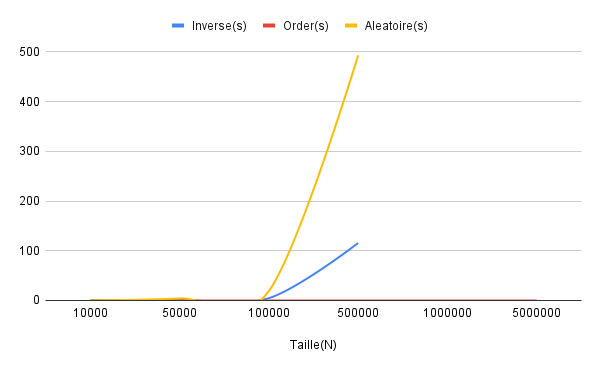
\includegraphics[scale=0.7]{ressources/bulleexp.png}
        \caption{Temps d'exécution du programme selon la taille du tableau}
    \label{fig:temps_exec_dico_theo}
\end{figure} 
\par
Depuis les graphes, on observe que le temps d’exécution évolue de manière quadratique avec l’augmentation de la taille du tableau pour le tri aleatoire et inverse , par contre il s'evolue de maniere linear dans la meilleur cas ( tableau tri en bon ordre) , ce qui correspond bien à la complexité théorique calculée auparavant.
\section{Conclusion}
A partir d'étude expérimentale et théorique de l'algorithme tri a bulle, On constate que malgré sa complexité en temps quadratique sur des données inversées ou triées aléatoirement, il est encore largement utilisé car il est capable de s'exécuter en temps linéaire sur des entrées déjà triées.
    
    \newpage
    \onehalfspacing
    \chapter{Tri par TAS}
\section {Description}
Il existe plusieurs types de méthodes de tri utilisées pour trier différents types de structures de données. L'une des méthodes de tri les plus populaires et les plus efficaces en informatique est le tri par tas.
\\
Le tri par tas  est une technique de tri basée sur la comparaison et basée sur la structure de données du tas.
\\
Tas (Heap en anglais) est une structure de données arborescente dans laquelle tous les nœuds de l'arbre sont dans un ordre spécifique. Tas est toujours un arbre binaire complet. 
\\
L'élément racine du Tas doit être à l'indice 0 dans le tableau.
\\
Pour le noeud à l'indice i :
\begin{itemize}
    \item  A l'indice (i-1)/2 se trouve le noeud parent.
    \item  A l'indice (2*i)+1, le nœud enfant gauche.
    \item  A l'index (2*i)+2, le noeud enfant de droite.
\end{itemize}


\section{Fonctionnement de l'algorithme}
L'algorithme du tri par tas fonctionne selon les étapes suivantes :
\begin{itemize}
 
     \item A partir des éléments du tableau donné, nous devons faire un tas maximum. Nous  commençons à empiler chaque sous-arbre de bas en haut et obtenir un max-heap après avoir appliqué la fonction à tous les éléments, y compris l'élément racine.
    \item  Retirer l'élément racine et le mettre à la fin du tableau (nième position) Mettre le dernier élément de l'arbre (tas) à la place vacante.
    \item  Réduire la taille du tas de 1.
    \item  Heapifier à nouveau l'élément racine de façon à avoir.
    \item l'élément le plus haut à la racine.
    \item Répétez ce processus encore et encore jusqu'à ce que tous les éléments de la liste soient triés dans le tableau avec succès.
\end{itemize}

\begin{figure}[H]
    \centering
        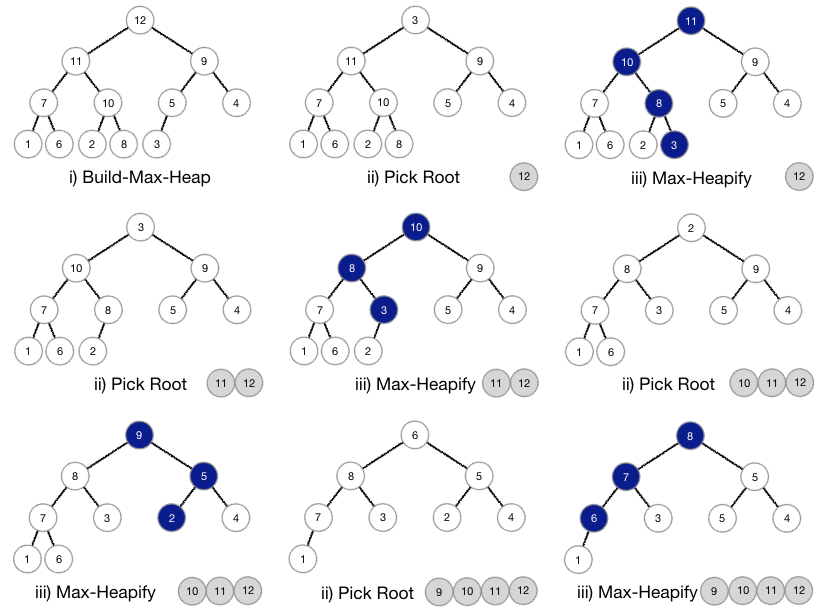
\includegraphics[scale=0.5]{ressources/HEAP.png}
        \caption{Exemple graphique d’un tri par tas}
    \label{fig:insert}
\end{figure}
Nous pouvons  représenter cet algorithme via le pseudo code suivant :
\par
\begin{function}[H]
    \textbf{Variables :}\\
    left,right : entier\;
    tmp,swapwith : entier\;
    
    
    \Begin{
        $left \leftarrow k*2-1 $\;
        $right \leftarrow k*2$\;
        $swapwith\leftarrow k-1 $\;
        \If{left<N et tab[left]>tab[swapwith]}
        {
               $swapwith\leftarrow left $\;
        }
        \If{right<N et tab[right]>tab[swapwith]}
        {
               $swapwith\leftarrow right $\;
        }
        \If{swapwith<>k-1}
        {
               $temp\leftarrow tab[swapwith] $\;
               $tab[swapwith]\leftarrow tab[k-1] $\;
               $tab[k-1] \leftarrow temp $\;
               heapify(tab,swapwith)\;
        }

      
    }
    \caption{heapify(Entrée: tab: tableau d'entier; k:entier;)}
\end{function}
\par
\begin{function}[H]
    \textbf{Variables :}\\
     temp,wn ,k: entier\;
    
    
    \Begin{
        \For{$k \leftarrow n/2$ \KwTo k>0}{
             heapify(tab,k)\; 
              $k\leftarrow k-1 $\;
         
            }
        \For{$wn \leftarrow n-1$ \KwTo wn>0}{
               $temp\leftarrow tab[0] $\;
               $tab[0]\leftarrow tab[wn] $\;
               $tab[wn] \leftarrow temp $\;
               heapify(tab,1)\;
            }
    }
    \caption{heapSort(Entrée: tab: tableau d'entier; )}
\end{function}
\section{Calcul de complexité}
\subsection{Complexité temporelle}
Heap Sort a des complexités temporelles O(nlog n) pour tous les cas (meilleur cas, cas moyen et pire cas).
\par
Dans la fonction heapify(), nous parcourons l'arbre de haut en bas. La hauteur d'un arbre binaire (la racine n'étant pas comptée) de taille n est log2 n au plus, c'est-à-dire que si le nombre d'éléments double, l'arbre ne devient plus profond que d'un niveau :
 \\
 \begin{figure}[H]
    \centering
        \includegraphics[scale=0.4]{ressources/complixité_tas.png}
        
    \label{fig:comtas}
\end{figure}

La complexité de la fonction heapify() est donc O(log n).
\\
\textbf{Complexité temporelle de la méthode HeapSort() :}

Pour construire initialement le tas, la méthode heapify () est appelée pour chaque nœud parent - en arrière, en commençant par le dernier nœud et en terminant à la racine de l'arbre.
\par
Un tas de taille n a n/2 nœuds parents (arrondis à l'inférieur) 
\par
La méthode heapify() est appelée n-1 fois. Ainsi, la complexité totale pour réparer le tas est également O(n log n).

\subsection{Complexité spatiale}
Étant donné que le tri en tas est un algorithme de tri conçu sur place, l'espace requis est constant, donc O (1). En effet, dans le cas de l'entrée :
\begin{enumerate}
  \item Nous utilisons la structure de tas pour organiser tous les éléments de la liste.
  \item Après avoir supprimé le plus grand nœud du tas max, nous plaçons l'élément supprimé à la fin de la même liste.
\end{enumerate}
Par conséquent, nous n'utilisons aucun espace supplémentaire lors de l'implémentation de cet algorithme. Cela donne à l'algorithme une complexité spatiale de O(1).
\\

\section{Experimentation}
Dans cette partie nous allons voir les résultats des exécutions de cet algorithme sur différents taille de tableau et sur données qui se représentent en 3 configuration ( triée en bon ordre , triée en ordre inverse , aléatoire) 
\subsubsection{Les données du tableau sont triées en bon ordre.}
\\
\begin{tabular}{| c | c | c | c | c | c | c | c | c | c | c |}
    \hline 
     Taille &  10000 & 50000 & 100000 & 500000 & 1000000 & 5000000 & 10000000 & 50000000 \\
    \hline
    temps(s) & 0,000066 &	0,000303	 & 0,000682	& 0,003029 & 0,00469 &	0,027033 & 0,062347 &	0,315974	 \\
   \hline
   
\end{tabular}
\par

\subsubsection{Les données du tableau sont triées en ordre inverse.}
\\
\begin{tabular}{| c | c | c | c | c | c | c | c | c | c | c |}
    \hline 
     Taille &  10000 & 50000 & 100000 & 500000 & 1000000 & 5000000 & 10000000 & 50000000 \\
    \hline
    temps(s) & 0,000052 &	0,00028 &	0,000643	 & 0,002413 &	0,005757 &	0,02379 &	0,049275 &	0,269919 \\
   
   \hline
\end{tabular}
\par
\subsubsection{Les données du tableau sont  positionnés aléatoirement.}
\\
\begin{tabular}{| c | c | c | c | c | c | c | c | c | c | c |}
    \hline 
     Taille &  10000 & 50000 & 100000 & 500000 & 1000000 & 5000000 & 10000000 & 50000000  \\
    \hline
    temps(s) & 0,000078 &	0,000384 &	0,000725	& 0,002596 &	0,004857 &	0,035832 &	0,057231 &	0,257452\\
    \hline
   
   
\end{tabular}
\par
\subsubsection{Le graphe :}
\\
La figure suivante représente les résultats d'exécution de cet algorithme selon les différentes taille du tableau.

\begin{figure}[H]
    \centering
        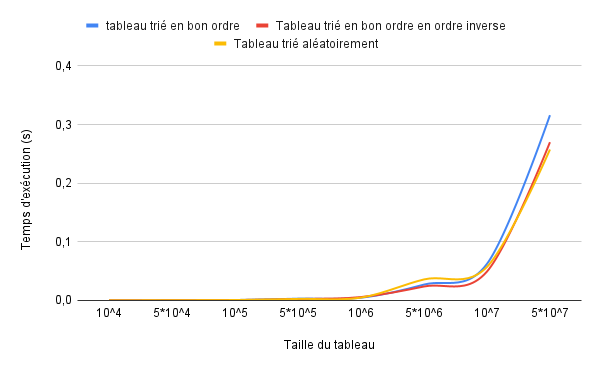
\includegraphics[scale=0.7]{ressources/heapchart.png}
        \caption{Temps d'execution du tri par tas sur les différents taille du tableau }
    \label{fig:insertch}
\end{figure}
\par
\par
D’après les graphes et les tableaux ci-dessus, Nous remarquons que le temps d’exécution évolue de manière quasi linéaire avec l’augmentation de la taille du tableau quel que soit sa configuration ( les 3 courbes sont presque  similaires) .
On en conclut que la complexité théorique est cohérente avec les résultats expérimentaux.

\section{Conclusion}
A partir d'étude expérimentale et théorique de l'algorithme tri par tas, On remarque que avec sa complexité temporelle de O(n log(n)) le tri en tas est toujours optimal. Il  a fonctionné avec succès sur les données  que nous avions prises et a obtenu des résultats satisfaisants pour les 3 configurations (table trié en ordre, table trié en inverse , table trié aleatoirement). 
    
    \newpage
    \onehalfspacing
    \chapter{Nombre Comparaisons}
Les tableau suivant représente les nombre de comparaison des algorithmes de tri selon la configuration du tableau.
\section{Tableau trie en bon ordre}
\small
\begin{center}
\resizebox{15cm}{!}{
\begin{tabular}{| c | c | c | c | c |  }
    \hline
     N &   10000 & 50000 & 10^5 & 5*10^5  \\
    \hline
    Tri par selection & 49995000 &	1249975000 &	4999950000 & 124999750000	 \\
    \hline
    Tri par insertion & 9999 & 49999 & 99999 & 499999\\
    \hline
    Tri par fusion & 1336310&	7844810&	16689460&	94757320	\\
    \hline
    Tri a bulle & 16588 &
56783 &
107007 &
508329  \\
    \hline
    Tri tas & 244460 & 1455438 & 3112517 & 17837785 		 \\
    \hline
    Tri rapide (Début) & 25005000 & 625025000 & 12500050000 & 62500250000\\
    \hline
    Tri rapide (Fin) & 49995001 & 1249975001& 4999950001 & 124999750001  \\
    \hline
    Tri rapide (Millieu) & 180011 & 1003409 & 2106802 & 11927156	 \\
    \hline
\end{tabular}}
\end{center}
\normalsize
La figure suivante représente l’évolution des nombres de comparaisons selon la taille du tableau 100000 
\begin{figure}[H]
    \centering
        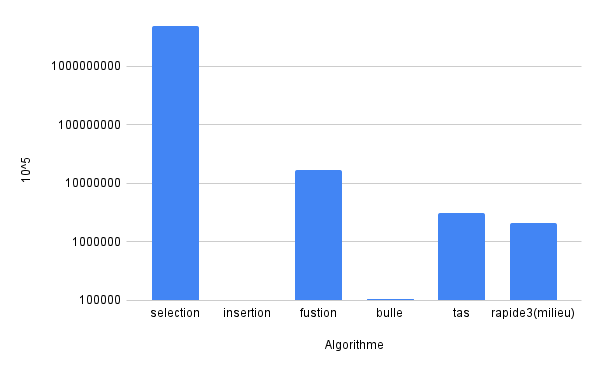
\includegraphics[scale=0.7]{ressources/comordre.png}
        \caption{nombre des comparaisons selon l'algorithme}
    \label{fig:temps_exec_dico_theo}
\end{figure} 
\par
Depuis le graphe, on observe que le nombre de comparaison dans la meilleur cas des algorithmes fusion , selection , tas et rapide est tres eleves par rapport aux algorithmes insertion et bulle.  
\par
\begin{figure}[H]
    \centering
        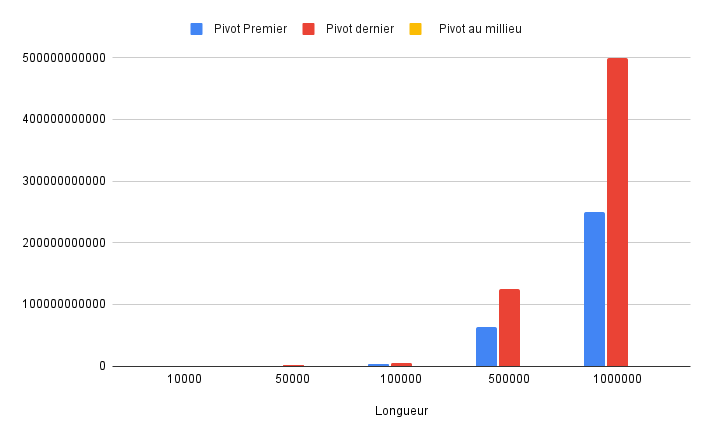
\includegraphics[scale=0.7]{ressources/nb_triee.png}
        \caption{Nombre des comparaisons effectuées par les  algorithmes de Tri Rapide selon la taille du tableau}
    \label{fig:temps_exec_dico_theo}
\end{figure} 
\par
\section{Tableau trie en ordre inverse}
\small
\begin{center}
\resizebox{15cm}{!}{
\begin{tabular}{| c | c | c | c | c |  }
    \hline
     N &   10000 & 50000 & 10^5 & 5*10^5  \\
    \hline
    Tri par selection & 49995000 &	1249975000	 & 4999950000 &	124999750000	 \\
    \hline
    Tri par insertion & 49995000 & 1249975000 & 4999950000 & 12499750000  \\
    \hline
    Tri par fusion & 1336310&	7844810&	16689460&	94757320	\\
    \hline
    Tri a bulle & 50001245 &
1250026893 &
5001098891 &
5001098891 	 \\
    \hline
    Tri tas &  226682 & 1366047 & 2926640 & 16977997   \\
    \hline
    Tri rapide (Début) & 50005000 & 1250025000 & 5000050000 & 125000250000  \\
    \hline
    Tri rapide (Fin) & 50005000 & 1250025000& 5000050000 & /  \\
    \hline
    Tri rapide (Millieu) & 143169 & 848331 & 1796637 & 9786465  \\
    \hline
\end{tabular}}
\end{center}
\normalsize
La figure suivante représente l’évolution du nombre de comparaisons selon l'algorithme utilisé avec une taille du tableau 100000 
\begin{figure}[H]
    \centering
        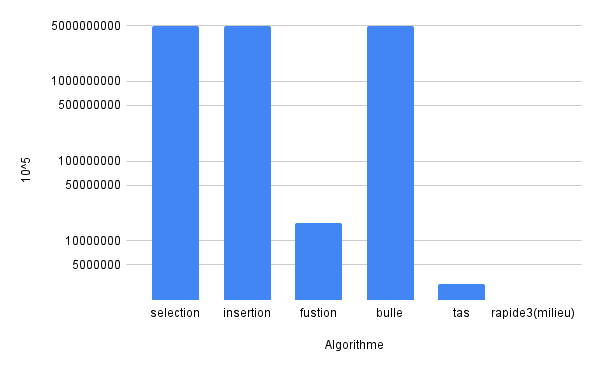
\includegraphics[scale=0.7]{ressources/cominverse.png}
        \caption{nombre des comparaisons selon l'algorithme}
    \label{fig:temps_exec_dico_theo}
\end{figure} 
\par
Depuis le graphe, on observe que le nombre de comparaison des algorithmes selection ,insertion et bulle est tres eleves par rapport aux autres algorithmes fusion , tas , et le tri rapide donnent des meilleurs resultats. 
\par
\begin{figure}[H]
    \centering
        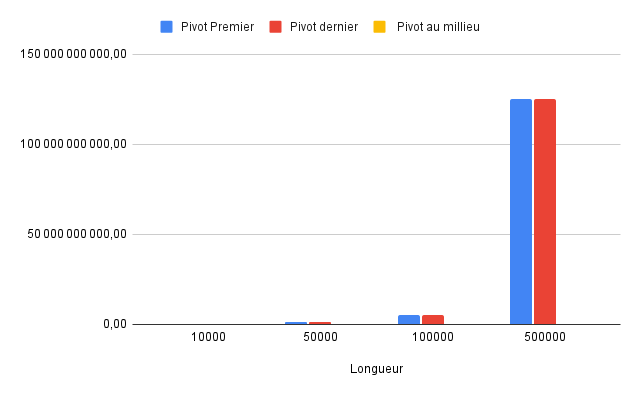
\includegraphics[scale=0.7]{ressources/nb_inv.png}
        \caption{Nombre des comparaisons effectuées par les  algorithmes de Tri Rapide selon la taille du tableau}
    \label{fig:temps_exec_dico_theo}
\end{figure} 
\par
\section{Tableau trie aleatoirement}
\small
\begin{center}
\resizebox{15cm}{!}{
\begin{tabular}{| c | c | c | c | c |  }
    \hline
     N &   10000 & 50000 & 10^5 & 5*10^5  \\
    \hline
    Tri par selection & 49995000 & 	1249975000	& 4999950000	& 124999750000	 \\
    \hline
    Tri par insertion & 25234406 &  623931087 & 2492077689 & 62470481149 \\
    \hline
    Tri par fusion & 1336310&	7844810&	16689460&	94757320		\\
    \hline
    Tri a bulle & 50002183 &
1250010338 &
5003278417 & //  \\
    \hline
    Tri tas &   235334 & 1409925 & 3019611 & 17397152   \\
    \hline
     Tri rapide (Début) & 161015 & 978870 & 12056258 & 11881598  \\
    \hline
    Tri rapide (Fin) & 168562 & 993500 & 2141419 & 12216452 	 \\
    \hline
    Tri rapide (Millieu) & 262726 & 1474652 & 3184007 & 18730250	 \\
    \hline
    
\end{tabular}}
\end{center}
\normalsize
La figure suivante représente l’évolution du nombre de comparaisons selon l'algorithme utilisé avec une taille du tableau 100000
\begin{figure}[H]
    \centering
        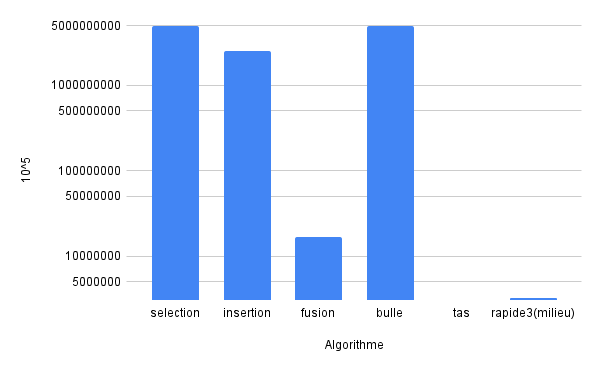
\includegraphics[scale=0.7]{ressources/comaleatoire.png}
        \caption{nombre des comparaisons selon l'algorithme}
    \label{fig:temps_exec_dico_theo}
\end{figure} 
\par
Depuis le graphe, on observe que le nombre de comparaison des algorithmes selection ,insertion et bulle est très elevés par rapport aux autres algorithmes fusion , rapide et tas avec meilleur complexite. 
\normalsize

\section{Conclusion}
depuis les graphes , on observe que le nombre des comparaisons represénte quasiment la complexité de l'algorithme ainsi qu'ils existent des algorithmes de comparaisons qui ne sont pas couteux en nombres de comparaisons effectuées et ils sont privilégiés dans la pratique dans le cas où la comparaison est dispendieuse.


    
    \newpage
    \onehalfspacing
    \chapter{Conclusion}
Beaucoup d'algorithmes existent, mais certains sont bien plus utilisés que d'autres en pratique. Le tri par insertion est souvent plébiscité pour des données de petite taille, tandis que des algorithmes asymptotiquement efficaces, comme le tri fusion, le tri par tas ou quicksort, seront utilisés pour des données de plus grande taille.
\\
La comparaison empirique d'algorithmes n'est pas aisée limitée au complexité de l'algorithme, il y'a beaucoup de paramètres entrent en compte : taille de données, ordre des données, matériel utilisé, taille de la mémoire vive, etc. 

    
    \newpage
    \onehalfspacing
    \chapter{Annexe :code source}
\section{Repartition des taches}
\par
\small
\resizebox{17cm}{!}{
\begin{tabular}{| c | c | }
    \hline
    Member &  Tache   \\
    \hline
    BEBNBACHIR Mohamed Amir & la conception de la solution iterative de hanoi + l'implementation en langage C + etude experimentale et analyse des resultats de la version iterative\\
    \hline
    BOUCHOUL Bouchra &  L'algorithme de verification avec calcule de sa complexite + Presentation d'une instance du probleme avec la solution (exemple)  \\
    \hline
    KHEMISSI Maroua &  Historique et presentation du probleme + Definition formelle du probleme+  Presentation de l'algorithme de resolution avec complexite theorique + representation de la modelisation de la solution\\
    \hline
    MEDJKOUNE Roumaissa & le programme de l'algorithme de résolution récursive en langage c + Son étude expérimentale + Analyse des résultats  \\
    \hline
  
\end{tabular}}
\\ \\
\newpage
\section{algorithme.c}
Le programme c 
\begin{minted}[
breaklines=true,
frame=lines,
linenos
]{c}
#include<stdio.h>
#include<stdlib.h>
#include<string.h>
#define MAX 100
#include<time.h>
//pile
struct discs {
	int size;
};
typedef discs *disc;
//les piles
typedef struct pile
{
    disc items[MAX];
    int top;
    int taille;
    int num;
} pile;

typedef struct Tour{
	int sizej;
	pile *A;
	pile *B;
	pile *C;
}Tour;
typedef Tour *TourH;


//les fonctions des piles
void initPile(pile *p,int num)
{
    p->top = -1;
    p->taille = 0;
    p->num=num;
}
int isempty(pile *p) {
   if (p->top == -1)
        return 1;
    else
        return 0;
}
int pilePleine(pile *s)
{
    if (s->top == MAX - 1)
        return 1;
    else
        return 0;
}
void push(pile *p, disc bt) {
 
    if (pilePleine(p))
    {
        printf("la pile est pleine");
    }
    else
    {
        p->top++;
        p->items[p->top] = bt;
    }
    p->taille++;

}
disc pop(pile *p) {
  if (isempty(p)){
  	return NULL;
  }
    p->taille--;
    disc val = p->items[p->top];
    p->top--;
    return val;
    }

///Initialiser le jeux en precisant le nombre initial des disques
TourH initHanoi(int size){
	TourH Tr= (TourH)malloc(sizeof(TourH));
	pile *A = (pile *)malloc(sizeof(pile));
    initPile(A,1);
    pile *B = (pile *)malloc(sizeof(pile));
    initPile(B,2);
    pile *C = (pile *)malloc(sizeof(pile));
    initPile(C,3);
    int i;
    for (i=size;i>0;i--){
    	disc d = (disc)malloc(sizeof(disc));
    	d->size=i;
    	push(A,d);
	}
    Tr->sizej=size;
    Tr->A=A;
    Tr->B=B;
    Tr->C=C;
 return Tr;
}

///fonction pou deplacer les disque entre les piles

void move(pile *p, pile *k,int* dep){
	disc d;
	d=pop(p);
	push(k,d);
	(*dep) += 1;
	
}

///fonctions tour d'hanoi
void Hanoi(int n,pile *A,pile *B,pile *C,int* dep){
	if (n>0){
	   Hanoi(n-1,A,C,B,dep);
	   move(A,C,dep);
	   Hanoi(n-1,B,A,C,dep);
	
	}
}

void moveI(pile * from ,pile * to){

    if (isempty(to))
    {
        push(to,pop(from));
    }
 
    else if (isempty(from))
    {
        push(from,pop(to));
    }
 
    else if (from->items[from->top]>to->items[to->top])
    {
        push(from,pop(to));
    }
 
    else
    {
        push(to,pop(from));
    }
}
void iterativeHanoi(int n,pile* start,pile* end,pile* inter){
    
    int total_num_of_moves = pow(2, n) - 1;
    
    
    if (n % 2 != 0)
    {
 
    for (int i = 1; i <= total_num_of_moves; i++)
    {
        if (i % 3 == 1)
        moveI(start,end);
 
        else if (i % 3 == 2)
        moveI(start,inter);
 
        else if (i % 3 == 0)
        moveI(inter,end);
    }
    }else{
        for (int i = 0; i < total_num_of_moves; i++)
    {
        if (i % 3 == 1)
        moveI(start,end);
 
        else if (i % 3 == 2)
        moveI(end,inter);
 
        else if (i % 3 == 0)
        moveI(inter,start);
    }
    }
}
void TourHanoi(TourH Tr,int* dep){
	Hanoi(Tr->sizej,Tr->A,Tr->B,Tr->C,dep);
}

int main(){
//enregistrement des executions

 clock_t t1,t2;
 double time;
 int j=5;
 FILE *f;
 f = fopen("nbDepHanoiRec.txt", "a");
  if (f != NULL)
    {  printf(" le fichier existe \n");}
    else
    { printf("Impossible d'ouvrir le fichier \n");}

 while(j<100){
     int d=0;
     TourH jeu= initHanoi(j);
     t1=clock();
     TourHanoi(jeu,&d);
     t2=clock();
     time=(float)(t2 - t1) / CLOCKS_PER_SEC;
     fprintf(f,"%d %d \n",j,d);
     j+=5;
 }


return 0;
}

\end{minted}
    
    \newpage
    \onehalfspacing
    \chapter{Références}
[1] Wikipedia .
\par
[2] Cours Algorithmique et Complexite - Prof DERIAS.H .



\end{document}